For the system of $N$ free fermions, we write the Hamiltonian $\hat{H}=\sum_\alpha E_\alpha\hat{a}^\dagger_\alpha\hat{a}_\alpha$ on $|\alpha\rangle$, a basis of a complete set of one-particle states, where the index labels the states by increasing order of energies, $E_1<E_2<\cdots$. Since we are dealing with fermions, we cannot put more than one particle in each state. Thus the state the lowest energy is obtained by filling up all the first $N$ single particle states. Let $|\text{gnd}\rangle$ denote this ground state.

$$|\text{gnd}\rangle\equiv|\overbrace{11\cdots 1}^N 00\cdots\rangle=\left(\prod_{\alpha=1}^N\hat{a}^\dagger_\alpha\right)|0\rangle$$

\noindent The energy of this state is $E_\text{gnd}=E_1+\cdots+E_N$. The energy of the top-most occupied single particle state $E_N$, is called the Fermi energy of the system and the set of occupied states is called the Fermi sea.\\

\noindent An excited state is obtained by removing one particle from the single particle state $N$ (thus leaving a hole behind) and putting the particle in the unoccupied single particle state $N+1$. This is a state with one particle-hole pair.

$$|\psi\rangle\equiv|\overbrace{11\cdots 1}^{N-1}0100\cdots\rangle=\hat{a}^\dagger_{N+1}\hat{a}_N|\text{gnd}\rangle$$

\noindent The energy of this state is $E_\psi=E_1+\cdots+E_{N-1}+E_{N+1}$. The excitation energy is $\varepsilon_\psi=E_\psi-E_\text{gnd}>0$.\\

\begin{center}
    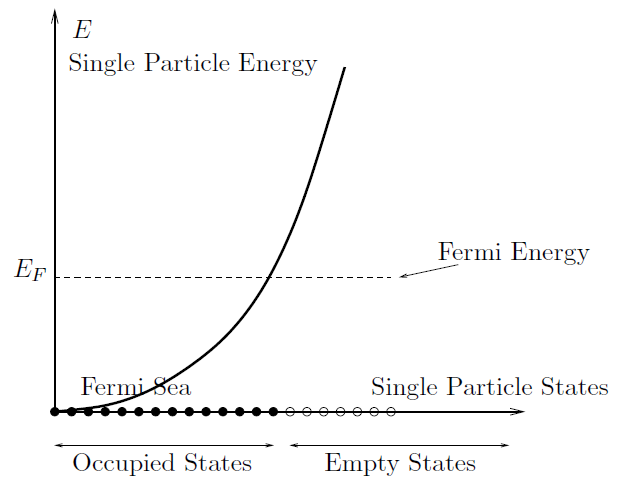
\includegraphics[scale=0.8]{fermi}
\end{center}

\noindent It is more reasonable to use $|\text{gnd}\rangle$ instead of $|0\rangle$ as the reference state. An operator $\hat{b}_\alpha=\hat{a}^\dagger_{\alpha}$ is introduced. Since these are fermionic operators, anticommutation relations $\{\hat{a}_{\alpha},\hat{a}^\dagger_{\alpha'}\}=\delta_{\alpha\alpha'}$ and $\{\hat{b}_{\beta},\hat{b}^\dagger_{\beta'}\}=\delta_{\beta\beta'}$ hold for $\alpha,\alpha'>N$ and $\beta,\beta'\leq N$.\\

\noindent Relative to the $|\text{gnd}\rangle$, $\hat{a}^\dagger_\alpha$ and $\hat{b}^\dagger_\beta$ behave like creation operators for electrons and holes respectively. An arbitrary excited state has the form

$$\hat{a}^\dagger_1\cdots\hat{a}^\dagger_m\hat{b}^\dagger_1\cdots\hat{b}^\dagger_n=|\alpha_1\cdots\alpha_m\beta_1\cdots\beta_n;\text{gnd}\rangle$$

\noindent This state has $m$ electrons and $n$ holes. $m$ is always equal to $n$. On the other hand, the ground state is annihilated by $\hat{a}_\alpha$ and $\hat{b}_\beta$.

$$\hat{a}_\alpha|\text{gnd}\rangle=\hat{b}_\beta|\text{gnd}\rangle=0$$\\

\noindent The Hamiltonian is normal ordered relative to the empty state, i.e. $\hat{H}|0\rangle=0$, but is not normal ordered relative to the ground state. The particle-hole transformation enables us to write,

$$\hat{H}=E_\text{gnd}+\sum_{\alpha>N}E_\alpha\hat{a}^\dagger_\alpha\hat{a}_\alpha-\sum_{\beta\leq N}E_\beta\hat{b}^\dagger_\beta\hat{b}_\beta$$

\noindent The number operator is given by

$$\hat{N}=N+\sum_{\alpha>N}\hat{a}^\dagger_\alpha\hat{a}_\alpha-\sum_{\beta\leq N}\hat{b}^\dagger_\beta\hat{b}_\beta$$

\noindent Electrons raise the energy while holes reduce it. Imposing the condition that the Hamiltonian conserves the particle number, i.e. $[\hat{N},\hat{H}]=0$, we see that for every particle that is removed a hole must be created. Hence particles and holes can only be created in pairs.